\section{Use Cases}

\begin{figure}[H]
    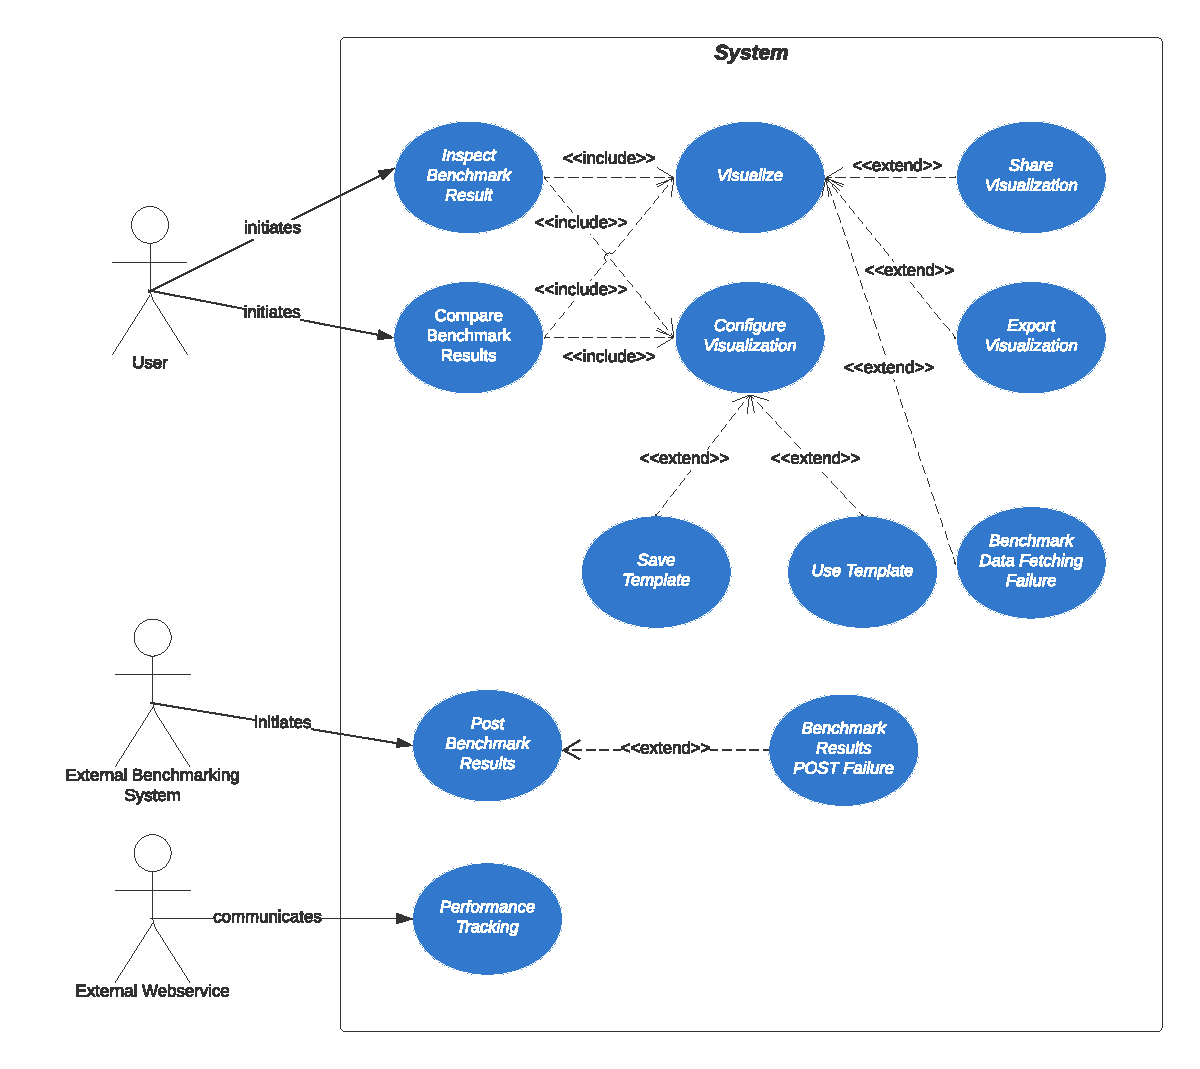
\includegraphics[width=\textwidth]{usecase}
    \caption{Use case diagram}
    \label{fig:usecase}
\end{figure}

\case{Plot}{cse:plot}
{Generating and displaying a Plot to a User}
{initiated by User}
{\gls{configuration} is available}
{\begin{enumerate}
    \item \parkview{} fetches the data specified in the \gls{configuration} from its database.
    \item \parkview{} takes the data and generates the \gls{plot} specified in the \gls{configuration}.
    \item The user gets redirected to a new site where he can inspect the generated \gls{plot}.
\end{enumerate}}
{The \gls{plot} specified by the \gls{configuration} gets shown to the user.}
\implementedby{scn:inspect-last-commit}{cse:plot}
\implementedby{scn:comp-benchmarks}{cse:plot}
\implementedby{scn:fetch-data-failure}{cse:plot}

\bigskip

\case{Configure Plot}{cse:config-vis}
{Configration of a \gls{plot}}
{initiated by User}
{User selected the \enquote{Create New Plot} option}
{\begin{enumerate}
    \item The configuration panel appears.
    \item The user chooses a \gls{plot type} and certain options that are specific to the \gls{plot type}, for example axis labels, plot title or compared dimensions.
\end{enumerate}}
{The \gls{configuration} gets updated.}
\implementedby{scn:inspect-last-commit}{cse:config-vis}
\implementedby{scn:comp-benchmarks}{cse:config-vis}
\implementedby{scn:fetch-data-failure}{cse:config-vis}

\bigskip

\case{Create New Plot}{cse:create-plot}
{Process for configuring and generating a plot}
{initated by User}
{\Gls{benchmark result} for commit is available}
{\begin{enumerate}
    \item The user selects one or more commits.
    \item The user initiates the \texttt{Configure Plot} use case by selecting the \enquote{Create New Plot} option.
    \item Once the user is satisfied with his \gls{configuration}, he initiates the \texttt{Plot} use case by selecting the \enquote{Create New Plot} option in the panel.
\end{enumerate}}
{Plot is displayed to the user}
\implementedby{scn:inspect-last-commit}{cse:create-plot}
\implementedby{scn:comp-benchmarks}{cse:create-plot}

\bigskip

\case{Post Benchmark Results}{cse:post-benchmark-res}
{An external \gls{benchmarking system} trying to upload \glspl{benchmark result}}
{initiated by External Benchmarking System}
{The external \gls{benchmarking system} ran the benchmarks}
{\begin{enumerate}
    \item \parkview{} receives a POST request containing \glspl{benchmark result}.
    \item \parkview{} converts the received data into the correct format.
    \item \parkview{} stores the received data in its database.
\end{enumerate}}
{The received performance data is stored in the database}
\implementedby{scn:perf-tracking}{cse:post-benchmark-res}
\implementedby{scn:post-data-failure}{cse:post-benchmark-res}

\bigskip

\caseOpt{Share Plot}{cse:share-vis}
{Sharing a \gls{plot} using a link}
{initiated by User}
{A \gls{plot} has been generated}
{\begin{enumerate}
    \item The user selects the \enquote{Share Plot} option.
    \item A link gets displayed.
    \item The link redirects any visitors to the same \gls{plot}.
\end{enumerate}}
{A link is shown which redirects to the \gls{plot}}
\implementedby{scn:share}{cse:share-vis}

\bigskip

\caseOpt{Export Plot}{cse:export-vis}
{Downloading a \gls{plot}}
{initiated by User}
{A \gls{plot} has been generated}
{\begin{enumerate}
    \item The user selects the \enquote{Export Plot} option.
    \item The user downloads the \gls{plot}.
\end{enumerate}}
{The User is offered a download of an export of the \gls{plot}}
\implementedby{scn:export}{cse:export-vis}

\bigskip

\caseOpt{Save Template}{cse:save-template}
{Storing a \gls{template} for later use}
{initiated by User}
{The user is in the \texttt{Configure Plot} use case}
{The \texttt{Save Template} use case extends the \texttt{Configure Plot} use case.
\begin{enumerate}
    \item The user selects the \enquote{save template} option.
    \item The user gets a \gls{json} download for his \gls{template}.
\end{enumerate}}
{\Gls{template} is stored locally}
\implementedby{scn:template}{cse:save-template}

\bigskip

\caseOpt{Use Template}{cse:use-temp}
{Using a previously created template}
{initiated by User}
{The user is in the \texttt{Configure Plot} use case and a \gls{template} is available locally}
{The \texttt{Use Template} use case extends the \texttt{Configure Plot} use case.
\begin{enumerate}
    \item The user selects the \enquote{use template} option.
    \item The user is prompted to upload a \gls{json} file containing the \gls{template}.
    \item The current \gls{configuration} options get set to the values specified in the \gls{template}.
\end{enumerate}}
{The \gls{template} is applied to the current configuration.}
\implementedby{scn:template}{cse:use-temp}

\bigskip

\caseOpt{Performance Tracking}{cse:perf-tracking}
{\parkview{} recognizes big changes in performance and notifies external webservices}
{communicates with External Webservice}
{New \glspl{benchmark result} has been posted to the backend}
{\begin{enumerate}
    \item \parkview{} evaluates the performance of the new \glspl{benchmark result}.
    \item \parkview{} compares the performance of the new benchmark with the performance of the corresponding benchmark of the last commit.
    \item \parkview{} relays the results to a configured number of hooks.
    \item The hooks contact their external webservices according to how they have been configured.
\end{enumerate}}
{\parkview{} fires a POST Request to all webhook subscribers}
\implementedby{scn:perf-tracking}{cse:perf-tracking}

\bigskip

\case{Benchmark Results POST Failure}{cse:benchmark-res-post-fail}
{Behavior in case of invalid POST request}
{communicates with External \Gls{benchmarking system}}
{The external \gls{benchmarking system} has sent a POST request}
{This use case extends the \texttt{Post Benchmark Results} use case if an error occurs.
\begin{enumerate}
    \item \parkview{} identifies the error.
    \item \parkview{} sends a response with the corresponding error code to the external \gls{benchmarking system}.
\end{enumerate}}
{Response is sent}
\implementedby{scn:post-data-failure}{cse:benchmark-res-post-fail}

\bigskip

\case{Benchmark Results Fetching Failure}{cse:benchmark-data-fetch-fail}
{Behavior in case of invalid request for \glspl{benchmark result}}
{displays error to User}
{This use case extends the \texttt{Plot} use case if an error occurs.}
{\begin{enumerate}
    \item \parkview{} identifies the error.
    \item \parkview{} displays an error message in the browser.
\end{enumerate}}
{Error message gets displayed}
\implementedby{scn:fetch-data-failure}{cse:benchmark-data-fetch-fail}

